% Options for packages loaded elsewhere
% Options for packages loaded elsewhere
\PassOptionsToPackage{unicode}{hyperref}
\PassOptionsToPackage{hyphens}{url}
\PassOptionsToPackage{dvipsnames,svgnames,x11names}{xcolor}
%
\documentclass[
  letterpaper,
  DIV=11,
  numbers=noendperiod]{scrartcl}
\usepackage{xcolor}
\usepackage{amsmath,amssymb}
\setcounter{secnumdepth}{-\maxdimen} % remove section numbering
\usepackage{iftex}
\ifPDFTeX
  \usepackage[T1]{fontenc}
  \usepackage[utf8]{inputenc}
  \usepackage{textcomp} % provide euro and other symbols
\else % if luatex or xetex
  \usepackage{unicode-math} % this also loads fontspec
  \defaultfontfeatures{Scale=MatchLowercase}
  \defaultfontfeatures[\rmfamily]{Ligatures=TeX,Scale=1}
\fi
\usepackage{lmodern}
\ifPDFTeX\else
  % xetex/luatex font selection
\fi
% Use upquote if available, for straight quotes in verbatim environments
\IfFileExists{upquote.sty}{\usepackage{upquote}}{}
\IfFileExists{microtype.sty}{% use microtype if available
  \usepackage[]{microtype}
  \UseMicrotypeSet[protrusion]{basicmath} % disable protrusion for tt fonts
}{}
\makeatletter
\@ifundefined{KOMAClassName}{% if non-KOMA class
  \IfFileExists{parskip.sty}{%
    \usepackage{parskip}
  }{% else
    \setlength{\parindent}{0pt}
    \setlength{\parskip}{6pt plus 2pt minus 1pt}}
}{% if KOMA class
  \KOMAoptions{parskip=half}}
\makeatother
% Make \paragraph and \subparagraph free-standing
\makeatletter
\ifx\paragraph\undefined\else
  \let\oldparagraph\paragraph
  \renewcommand{\paragraph}{
    \@ifstar
      \xxxParagraphStar
      \xxxParagraphNoStar
  }
  \newcommand{\xxxParagraphStar}[1]{\oldparagraph*{#1}\mbox{}}
  \newcommand{\xxxParagraphNoStar}[1]{\oldparagraph{#1}\mbox{}}
\fi
\ifx\subparagraph\undefined\else
  \let\oldsubparagraph\subparagraph
  \renewcommand{\subparagraph}{
    \@ifstar
      \xxxSubParagraphStar
      \xxxSubParagraphNoStar
  }
  \newcommand{\xxxSubParagraphStar}[1]{\oldsubparagraph*{#1}\mbox{}}
  \newcommand{\xxxSubParagraphNoStar}[1]{\oldsubparagraph{#1}\mbox{}}
\fi
\makeatother

\usepackage{color}
\usepackage{fancyvrb}
\newcommand{\VerbBar}{|}
\newcommand{\VERB}{\Verb[commandchars=\\\{\}]}
\DefineVerbatimEnvironment{Highlighting}{Verbatim}{commandchars=\\\{\}}
% Add ',fontsize=\small' for more characters per line
\usepackage{framed}
\definecolor{shadecolor}{RGB}{241,243,245}
\newenvironment{Shaded}{\begin{snugshade}}{\end{snugshade}}
\newcommand{\AlertTok}[1]{\textcolor[rgb]{0.68,0.00,0.00}{#1}}
\newcommand{\AnnotationTok}[1]{\textcolor[rgb]{0.37,0.37,0.37}{#1}}
\newcommand{\AttributeTok}[1]{\textcolor[rgb]{0.40,0.45,0.13}{#1}}
\newcommand{\BaseNTok}[1]{\textcolor[rgb]{0.68,0.00,0.00}{#1}}
\newcommand{\BuiltInTok}[1]{\textcolor[rgb]{0.00,0.23,0.31}{#1}}
\newcommand{\CharTok}[1]{\textcolor[rgb]{0.13,0.47,0.30}{#1}}
\newcommand{\CommentTok}[1]{\textcolor[rgb]{0.37,0.37,0.37}{#1}}
\newcommand{\CommentVarTok}[1]{\textcolor[rgb]{0.37,0.37,0.37}{\textit{#1}}}
\newcommand{\ConstantTok}[1]{\textcolor[rgb]{0.56,0.35,0.01}{#1}}
\newcommand{\ControlFlowTok}[1]{\textcolor[rgb]{0.00,0.23,0.31}{\textbf{#1}}}
\newcommand{\DataTypeTok}[1]{\textcolor[rgb]{0.68,0.00,0.00}{#1}}
\newcommand{\DecValTok}[1]{\textcolor[rgb]{0.68,0.00,0.00}{#1}}
\newcommand{\DocumentationTok}[1]{\textcolor[rgb]{0.37,0.37,0.37}{\textit{#1}}}
\newcommand{\ErrorTok}[1]{\textcolor[rgb]{0.68,0.00,0.00}{#1}}
\newcommand{\ExtensionTok}[1]{\textcolor[rgb]{0.00,0.23,0.31}{#1}}
\newcommand{\FloatTok}[1]{\textcolor[rgb]{0.68,0.00,0.00}{#1}}
\newcommand{\FunctionTok}[1]{\textcolor[rgb]{0.28,0.35,0.67}{#1}}
\newcommand{\ImportTok}[1]{\textcolor[rgb]{0.00,0.46,0.62}{#1}}
\newcommand{\InformationTok}[1]{\textcolor[rgb]{0.37,0.37,0.37}{#1}}
\newcommand{\KeywordTok}[1]{\textcolor[rgb]{0.00,0.23,0.31}{\textbf{#1}}}
\newcommand{\NormalTok}[1]{\textcolor[rgb]{0.00,0.23,0.31}{#1}}
\newcommand{\OperatorTok}[1]{\textcolor[rgb]{0.37,0.37,0.37}{#1}}
\newcommand{\OtherTok}[1]{\textcolor[rgb]{0.00,0.23,0.31}{#1}}
\newcommand{\PreprocessorTok}[1]{\textcolor[rgb]{0.68,0.00,0.00}{#1}}
\newcommand{\RegionMarkerTok}[1]{\textcolor[rgb]{0.00,0.23,0.31}{#1}}
\newcommand{\SpecialCharTok}[1]{\textcolor[rgb]{0.37,0.37,0.37}{#1}}
\newcommand{\SpecialStringTok}[1]{\textcolor[rgb]{0.13,0.47,0.30}{#1}}
\newcommand{\StringTok}[1]{\textcolor[rgb]{0.13,0.47,0.30}{#1}}
\newcommand{\VariableTok}[1]{\textcolor[rgb]{0.07,0.07,0.07}{#1}}
\newcommand{\VerbatimStringTok}[1]{\textcolor[rgb]{0.13,0.47,0.30}{#1}}
\newcommand{\WarningTok}[1]{\textcolor[rgb]{0.37,0.37,0.37}{\textit{#1}}}

\usepackage{longtable,booktabs,array}
\usepackage{calc} % for calculating minipage widths
% Correct order of tables after \paragraph or \subparagraph
\usepackage{etoolbox}
\makeatletter
\patchcmd\longtable{\par}{\if@noskipsec\mbox{}\fi\par}{}{}
\makeatother
% Allow footnotes in longtable head/foot
\IfFileExists{footnotehyper.sty}{\usepackage{footnotehyper}}{\usepackage{footnote}}
\makesavenoteenv{longtable}
\usepackage{graphicx}
\makeatletter
\newsavebox\pandoc@box
\newcommand*\pandocbounded[1]{% scales image to fit in text height/width
  \sbox\pandoc@box{#1}%
  \Gscale@div\@tempa{\textheight}{\dimexpr\ht\pandoc@box+\dp\pandoc@box\relax}%
  \Gscale@div\@tempb{\linewidth}{\wd\pandoc@box}%
  \ifdim\@tempb\p@<\@tempa\p@\let\@tempa\@tempb\fi% select the smaller of both
  \ifdim\@tempa\p@<\p@\scalebox{\@tempa}{\usebox\pandoc@box}%
  \else\usebox{\pandoc@box}%
  \fi%
}
% Set default figure placement to htbp
\def\fps@figure{htbp}
\makeatother





\setlength{\emergencystretch}{3em} % prevent overfull lines

\providecommand{\tightlist}{%
  \setlength{\itemsep}{0pt}\setlength{\parskip}{0pt}}



 


\KOMAoption{captions}{tableheading}
\makeatletter
\@ifpackageloaded{caption}{}{\usepackage{caption}}
\AtBeginDocument{%
\ifdefined\contentsname
  \renewcommand*\contentsname{Table of contents}
\else
  \newcommand\contentsname{Table of contents}
\fi
\ifdefined\listfigurename
  \renewcommand*\listfigurename{List of Figures}
\else
  \newcommand\listfigurename{List of Figures}
\fi
\ifdefined\listtablename
  \renewcommand*\listtablename{List of Tables}
\else
  \newcommand\listtablename{List of Tables}
\fi
\ifdefined\figurename
  \renewcommand*\figurename{Figure}
\else
  \newcommand\figurename{Figure}
\fi
\ifdefined\tablename
  \renewcommand*\tablename{Table}
\else
  \newcommand\tablename{Table}
\fi
}
\@ifpackageloaded{float}{}{\usepackage{float}}
\floatstyle{ruled}
\@ifundefined{c@chapter}{\newfloat{codelisting}{h}{lop}}{\newfloat{codelisting}{h}{lop}[chapter]}
\floatname{codelisting}{Listing}
\newcommand*\listoflistings{\listof{codelisting}{List of Listings}}
\makeatother
\makeatletter
\makeatother
\makeatletter
\@ifpackageloaded{caption}{}{\usepackage{caption}}
\@ifpackageloaded{subcaption}{}{\usepackage{subcaption}}
\makeatother
\usepackage{bookmark}
\IfFileExists{xurl.sty}{\usepackage{xurl}}{} % add URL line breaks if available
\urlstyle{same}
\hypersetup{
  pdftitle={MRP Estimation of State-Level Trust in Public Schools},
  colorlinks=true,
  linkcolor={blue},
  filecolor={Maroon},
  citecolor={Blue},
  urlcolor={Blue},
  pdfcreator={LaTeX via pandoc}}


\title{MRP Estimation of State-Level Trust in Public Schools}
\author{}
\date{}
\begin{document}
\maketitle


\subsection{Overview:}\label{overview}

My goal was to produce state-level estimates of institutional trust in
public schools, using MRP to produce (hopefully) better estimates. I
built the pipelines from 4 data sources:\\
- The YouGov baseline from 11/21/24 (with n of about 58k for this
question)\\
- ACS 2023
(https://www.census.gov/programs-surveys/acs/microdata.html)\\
- CCES Cumulative from 2021-2024 (https://doi.org/10.7910/DVN/II2DB6)\\
- 2024 FEC Presidential Election Results
(https://www.fec.gov/introduction-campaign-finance/election-results-and-voting-information/)

Due to the ACS survey not containing information on party ID, I used a
synthetic joint distribution adapted from Shiro Kuriwaki's package
(https://github.com/kuriwaki/synthjoint/). As outputs, I produced 3 sets
of estimates, a baseline built without party ID from MRP on demographics
alone, and then 2 variations with party ID using 2 different synthetic
joint distribution methods.

\subsection{Results:}\label{results}

I ran some comparisons between weighted survey mean and MRP, those
results are at the bottom of this doc

\subsubsection{Regression:}\label{regression}

Here are the summary tables for the regressions w/ base and pid.

\begin{Shaded}
\begin{Highlighting}[]
\FunctionTok{summary}\NormalTok{(base\_model)}
\end{Highlighting}
\end{Shaded}

\begin{verbatim}
Loading required namespace: rstan
\end{verbatim}

\begin{verbatim}
 Family: bernoulli 
  Links: mu = logit 
Formula: trust_schools_binary ~ sex_mrp + (1 | age_mrp) + (1 | educ_mrp) + (1 | race_mrp) + (1 | STATE) + (1 | STATE:educ_mrp) + (1 | STATE:race_mrp) 
   Data: rivers_cleaner_df (Number of observations: 62425) 
  Draws: 4 chains, each with iter = 2000; warmup = 1000; thin = 1;
         total post-warmup draws = 4000

Multilevel Hyperparameters:
~age_mrp (Number of levels: 4) 
              Estimate Est.Error l-95% CI u-95% CI Rhat Bulk_ESS Tail_ESS
sd(Intercept)     0.32      0.20     0.12     0.84 1.00     2238     2960

~educ_mrp (Number of levels: 4) 
              Estimate Est.Error l-95% CI u-95% CI Rhat Bulk_ESS Tail_ESS
sd(Intercept)     0.51      0.28     0.21     1.26 1.00     2083     2373

~race_mrp (Number of levels: 5) 
              Estimate Est.Error l-95% CI u-95% CI Rhat Bulk_ESS Tail_ESS
sd(Intercept)     0.35      0.17     0.16     0.81 1.00     2045     2489

~STATE (Number of levels: 51) 
              Estimate Est.Error l-95% CI u-95% CI Rhat Bulk_ESS Tail_ESS
sd(Intercept)     0.15      0.03     0.09     0.21 1.00     1391     1465

~STATE:educ_mrp (Number of levels: 204) 
              Estimate Est.Error l-95% CI u-95% CI Rhat Bulk_ESS Tail_ESS
sd(Intercept)     0.07      0.02     0.03     0.10 1.01      915     1071

~STATE:race_mrp (Number of levels: 251) 
              Estimate Est.Error l-95% CI u-95% CI Rhat Bulk_ESS Tail_ESS
sd(Intercept)     0.11      0.02     0.07     0.15 1.00     1447     2227

Regression Coefficients:
             Estimate Est.Error l-95% CI u-95% CI Rhat Bulk_ESS Tail_ESS
Intercept       -0.48      0.34    -1.15     0.21 1.00     2296     2674
sex_mrpWoman     0.02      0.02    -0.01     0.05 1.00    10475     3255

Draws were sampled using sample(hmc). For each parameter, Bulk_ESS
and Tail_ESS are effective sample size measures, and Rhat is the potential
scale reduction factor on split chains (at convergence, Rhat = 1).
\end{verbatim}

\begin{Shaded}
\begin{Highlighting}[]
\FunctionTok{summary}\NormalTok{(pid\_model)}
\end{Highlighting}
\end{Shaded}

\begin{verbatim}
 Family: bernoulli 
  Links: mu = logit 
Formula: trust_schools_binary ~ sex_mrp + pid3_mrp + (1 | age_mrp) + (1 | educ_mrp) + (1 | race_mrp) + (1 | STATE) + (1 | STATE:educ_mrp) + (1 | STATE:race_mrp) + trump_z 
   Data: rivers_cleaner_synth (Number of observations: 58484) 
  Draws: 4 chains, each with iter = 2000; warmup = 1000; thin = 1;
         total post-warmup draws = 4000

Multilevel Hyperparameters:
~age_mrp (Number of levels: 4) 
              Estimate Est.Error l-95% CI u-95% CI Rhat Bulk_ESS Tail_ESS
sd(Intercept)     0.31      0.20     0.12     0.84 1.00     2022     2455

~educ_mrp (Number of levels: 4) 
              Estimate Est.Error l-95% CI u-95% CI Rhat Bulk_ESS Tail_ESS
sd(Intercept)     0.38      0.25     0.14     1.08 1.00     1731     2538

~race_mrp (Number of levels: 5) 
              Estimate Est.Error l-95% CI u-95% CI Rhat Bulk_ESS Tail_ESS
sd(Intercept)     0.31      0.17     0.14     0.74 1.00     1883     2440

~STATE (Number of levels: 51) 
              Estimate Est.Error l-95% CI u-95% CI Rhat Bulk_ESS Tail_ESS
sd(Intercept)     0.13      0.03     0.06     0.20 1.01      764      589

~STATE:educ_mrp (Number of levels: 204) 
              Estimate Est.Error l-95% CI u-95% CI Rhat Bulk_ESS Tail_ESS
sd(Intercept)     0.05      0.02     0.01     0.09 1.00      600      503

~STATE:race_mrp (Number of levels: 250) 
              Estimate Est.Error l-95% CI u-95% CI Rhat Bulk_ESS Tail_ESS
sd(Intercept)     0.10      0.03     0.05     0.15 1.00      844     1445

Regression Coefficients:
                    Estimate Est.Error l-95% CI u-95% CI Rhat Bulk_ESS Tail_ESS
Intercept               0.27      0.31    -0.30     0.94 1.00     1852     2121
sex_mrpWoman           -0.14      0.02    -0.18    -0.11 1.00     7665     2883
pid3_mrpIndependent    -1.00      0.02    -1.05    -0.96 1.00     7038     3219
pid3_mrpRepublican     -1.54      0.02    -1.59    -1.49 1.00     7201     3300
trump_z                 0.01      0.06    -0.10     0.13 1.00     3674     2696

Draws were sampled using sample(hmc). For each parameter, Bulk_ESS
and Tail_ESS are effective sample size measures, and Rhat is the potential
scale reduction factor on split chains (at convergence, Rhat = 1).
\end{verbatim}

Essentially, partisanship dominated. Republicans and Independents have
massively negative log-odds compared to Democrats. The most major change
between the baseline and pid was sex. Without pid, women were about 0,
while after controlling for partisanship, they had -0.14 log odds.

One very interesting thing was that the vote share for Trump had
essentially no effect, which suggests that red and blue states don't
matter beyond individual party ID. Essentially, this would suggest a
Republican in California is as roughly as likely to trust public schools
as one in Alabama.

\subsubsection{State estimates:}\label{state-estimates}

\paragraph{Table}\label{table}

\begin{longtable}[]{@{}llll@{}}
\caption{Trust in Public Schools: MRP Estimates and Survey
Means}\tabularnewline
\toprule\noalign{}
State & BMLogit (PID) & Baseline & Survey (Raw) \\
\midrule\noalign{}
\endfirsthead
\toprule\noalign{}
State & BMLogit (PID) & Baseline & Survey (Raw) \\
\midrule\noalign{}
\endhead
\bottomrule\noalign{}
\endlastfoot
D.C. & 46.9\% ± 6.0 & 42.1\% ± 5.7 & 50.5\% \\
Massachusetts & 43.4\% ± 2.7 & 43.4\% ± 2.7 & 40.6\% \\
Iowa & 43.4\% ± 3.5 & 44.2\% ± 3.6 & 43.0\% \\
New Jersey & 42.5\% ± 2.4 & 42.2\% ± 2.6 & 42.7\% \\
Connecticut & 42.2\% ± 3.2 & 42.9\% ± 3.4 & 41.0\% \\
Nebraska & 41.9\% ± 4.2 & 43.8\% ± 4.3 & 41.5\% \\
Minnesota & 41.7\% ± 2.6 & 43.1\% ± 2.8 & 38.3\% \\
Utah & 40.8\% ± 3.6 & 41.0\% ± 3.8 & 41.0\% \\
California & 40.6\% ± 1.6 & 40.2\% ± 1.7 & 43.9\% \\
Colorado & 40.4\% ± 2.6 & 40.6\% ± 2.7 & 34.8\% \\
New York & 40.4\% ± 1.6 & 40.9\% ± 1.7 & 44.2\% \\
Kansas & 40.2\% ± 3.6 & 42.2\% ± 3.7 & 39.1\% \\
Maine & 39.8\% ± 4.1 & 41.5\% ± 4.4 & 33.5\% \\
Vermont & 39.5\% ± 5.5 & 39.5\% ± 5.7 & 37.7\% \\
Virginia & 39.2\% ± 2.3 & 37.7\% ± 2.3 & 35.9\% \\
Michigan & 39.0\% ± 2.1 & 39.7\% ± 2.2 & 35.1\% \\
Wisconsin & 38.6\% ± 2.5 & 40.7\% ± 2.6 & 33.0\% \\
New Hampshire & 38.6\% ± 4.0 & 38.3\% ± 4.3 & 31.4\% \\
Rhode Island & 38.5\% ± 4.8 & 37.5\% ± 5.0 & 40.2\% \\
Maryland & 38.2\% ± 2.8 & 38.2\% ± 2.9 & 34.7\% \\
Washington & 38.2\% ± 2.3 & 39.7\% ± 2.3 & 38.2\% \\
Montana & 37.9\% ± 4.4 & 38.7\% ± 4.8 & 26.0\% \\
Illinois & 37.5\% ± 2.1 & 37.7\% ± 2.1 & 37.1\% \\
Georgia & 37.3\% ± 2.0 & 37.2\% ± 2.2 & 39.8\% \\
Texas & 37.2\% ± 1.7 & 36.9\% ± 1.8 & 38.2\% \\
Arkansas & 37.0\% ± 3.6 & 36.5\% ± 3.5 & 35.6\% \\
Pennsylvania & 36.7\% ± 1.8 & 37.0\% ± 1.8 & 33.5\% \\
Oregon & 36.7\% ± 2.6 & 37.7\% ± 2.7 & 36.4\% \\
Mississippi & 36.6\% ± 4.0 & 35.2\% ± 4.3 & 32.8\% \\
Wyoming & 36.4\% ± 5.7 & 36.9\% ± 6.2 & 28.3\% \\
Ohio & 36.4\% ± 1.9 & 37.2\% ± 1.9 & 33.0\% \\
North Carolina & 36.1\% ± 2.1 & 35.9\% ± 2.2 & 30.8\% \\
South Dakota & 36.0\% ± 5.1 & 39.0\% ± 5.4 & 40.5\% \\
Florida & 35.9\% ± 1.6 & 35.5\% ± 1.6 & 35.0\% \\
Kentucky & 35.7\% ± 2.9 & 37.2\% ± 3.1 & 31.1\% \\
North Dakota & 35.4\% ± 5.3 & 37.3\% ± 5.9 & 38.8\% \\
Indiana & 35.1\% ± 2.5 & 34.6\% ± 2.7 & 33.9\% \\
Delaware & 35.1\% ± 4.4 & 34.8\% ± 4.6 & 36.0\% \\
New Mexico & 34.7\% ± 3.8 & 33.2\% ± 3.9 & 34.1\% \\
Arizona & 34.5\% ± 2.3 & 34.0\% ± 2.4 & 30.5\% \\
Hawaii & 34.3\% ± 4.6 & 34.7\% ± 5.2 & 31.3\% \\
Alaska & 33.9\% ± 4.9 & 35.6\% ± 5.2 & 46.2\% \\
Missouri & 33.9\% ± 2.4 & 34.2\% ± 2.5 & 30.7\% \\
South Carolina & 33.5\% ± 2.7 & 33.2\% ± 2.8 & 33.2\% \\
Nevada & 33.3\% ± 3.3 & 32.2\% ± 3.3 & 36.0\% \\
Tennessee & 33.2\% ± 2.5 & 32.9\% ± 2.6 & 28.6\% \\
Idaho & 33.0\% ± 4.1 & 32.4\% ± 4.2 & 26.8\% \\
Alabama & 30.5\% ± 2.9 & 29.7\% ± 3.0 & 29.8\% \\
Oklahoma & 30.5\% ± 3.0 & 30.6\% ± 3.1 & 23.2\% \\
West Virginia & 30.2\% ± 3.7 & 31.9\% ± 3.9 & 23.6\% \\
Louisiana & 29.4\% ± 3.3 & 28.2\% ± 3.4 & 23.1\% \\
\end{longtable}

\paragraph{Map}\label{map}

\pandocbounded{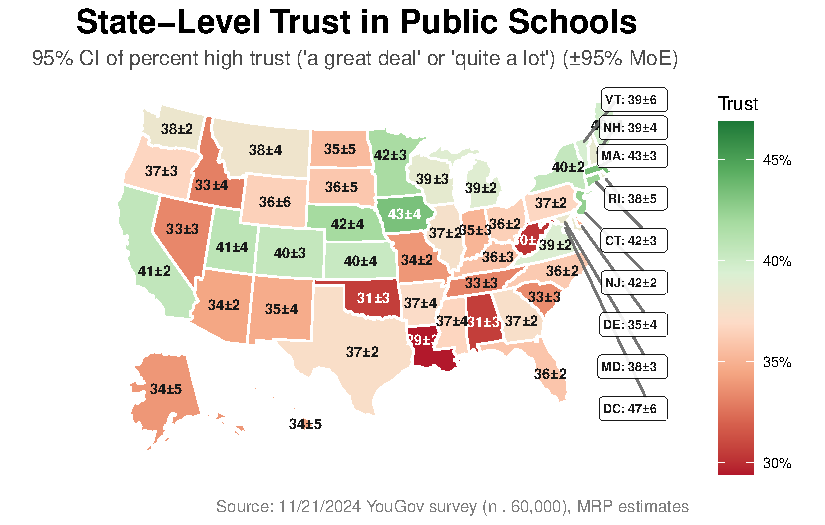
\includegraphics[keepaspectratio]{StateMRPpublicschools_files/figure-pdf/Map-1.pdf}}

\subsection{Data:}\label{data}

\subsubsection{For institutional trust:}\label{for-institutional-trust}

Trust in public schools binned into high (``A great deal'' and ``Quite a
lot'') and low (``Some'' and ``Very little''), leaving 58,000
respondents.

\subsubsection{For demographics:}\label{for-demographics}

\begin{itemize}
\tightlist
\item
  standard 4 group age (``Under 30'', ``30-44'', ``45-64'', ``65+'')
\item
  standard 4 group education (``HS or less'', ``Some college'',
  ``College grad'', ``Postgrad'')
\item
  5 group race ( ``Hispanic'', ``White'', ``Black'', ``Asian'',
  ``Other'')
\item
  sex/gender (``Man'', ``Woman'')
\end{itemize}

\subsubsection{For party ID:}\label{for-party-id}

\begin{itemize}
\tightlist
\item
  pid3 (``Democrat'', ``Republican'', ``Independent'') used from YouGov
\item
  state marginals drawn from CCES pooled across 2021-2024
\end{itemize}

\subsubsection{State context:}\label{state-context}

To differentiate pid3 and stablize across states, I wanted to add a
secondary variable at the state level to account for differences in
party identification at state level, so I added the z-score of the Trump
2024 vote share.

\subsection{Methods:}\label{methods}

\subsubsection{Synthetic joint:}\label{synthetic-joint}

ACS has no partisanship, so had to use a synthetic joint distribution to
poststratify on it. There are a few different ways of doing this, but
they tend to either use an outside data source to find marginals or rely
solely on the survey itself. To correct for the sampling bias of the
YouGov survey, I used weighted CCES with its representative pid category
as the marginals.

The two best synthetic joint methods for data of this scale are
smoothfix, which rakes the ACS uniformly to hit CCES partisan marginals
(which of course assumes independence) and bmlogit, a multinomial model
which uses the survey data to learn partisan to demographic
relationships and then reweights those to match CCES marginals. I
decided to run both and the answer was they were essentially the same w/
r \textgreater{} 0.99, though bmlogit is methodologically cleaner. Here
are the correlations at the cell level and in the final mrp results:

\begin{Shaded}
\begin{Highlighting}[]
\CommentTok{\# Cell level}
\FunctionTok{cor}\NormalTok{(frame\_bm}\SpecialCharTok{$}\NormalTok{count, frame\_smfx}\SpecialCharTok{$}\NormalTok{count)}
\end{Highlighting}
\end{Shaded}

\begin{verbatim}
[1] 0.991912
\end{verbatim}

\begin{Shaded}
\begin{Highlighting}[]
\CommentTok{\# Final MRP results}
\FunctionTok{cor}\NormalTok{(mrp\_bm}\SpecialCharTok{$}\NormalTok{p\_mrp\_est, mrp\_smfx}\SpecialCharTok{$}\NormalTok{p\_mrp\_est)}
\end{Highlighting}
\end{Shaded}

\begin{verbatim}
[1] 0.9905192
\end{verbatim}

Both were highly correlated with the (no pid) baseline, but not to the
same degree.

\begin{Shaded}
\begin{Highlighting}[]
\CommentTok{\# with pid vs. baseline}
\FunctionTok{cor}\NormalTok{(mrp\_bm}\SpecialCharTok{$}\NormalTok{p\_mrp\_est, mrp\_base}\SpecialCharTok{$}\NormalTok{p\_mrp\_est)}
\end{Highlighting}
\end{Shaded}

\begin{verbatim}
[1] 0.9450402
\end{verbatim}

\subsubsection{MRP Model:}\label{mrp-model}

I adapted my workflow from Kuriwaki's ccesMRPrun
(https://github.com/kuriwaki/ccesMRPrun) and ccesMRPprep
(https://github.com/kuriwaki/ccesMRPprep) packages. For my regression
formulas, I used:

\begin{Shaded}
\begin{Highlighting}[]
\CommentTok{\# baseline}
\NormalTok{formula\_baseline }\OtherTok{\textless{}{-}}\NormalTok{ trust\_schools\_binary }\SpecialCharTok{\textasciitilde{}}\NormalTok{  sex\_mrp }\SpecialCharTok{+} 
\NormalTok{  (}\DecValTok{1}\SpecialCharTok{|}\NormalTok{age\_mrp) }\SpecialCharTok{+}\NormalTok{ (}\DecValTok{1}\SpecialCharTok{|}\NormalTok{educ\_mrp) }\SpecialCharTok{+}\NormalTok{ (}\DecValTok{1}\SpecialCharTok{|}\NormalTok{race\_mrp) }\SpecialCharTok{+}\NormalTok{ (}\DecValTok{1}\SpecialCharTok{|}\NormalTok{STATE) }\SpecialCharTok{+}
\NormalTok{  (}\DecValTok{1} \SpecialCharTok{|}\NormalTok{ STATE}\SpecialCharTok{:}\NormalTok{educ\_mrp) }\SpecialCharTok{+}\NormalTok{ (}\DecValTok{1} \SpecialCharTok{|}\NormalTok{ STATE}\SpecialCharTok{:}\NormalTok{race\_mrp)}

\CommentTok{\# with PID}
\NormalTok{formula\_partisan }\OtherTok{\textless{}{-}}\NormalTok{ trust\_schools\_binary }\SpecialCharTok{\textasciitilde{}}\NormalTok{  sex\_mrp }\SpecialCharTok{+}\NormalTok{ pid3\_mrp }\SpecialCharTok{+} 
\NormalTok{  (}\DecValTok{1}\SpecialCharTok{|}\NormalTok{age\_mrp) }\SpecialCharTok{+}\NormalTok{ (}\DecValTok{1}\SpecialCharTok{|}\NormalTok{educ\_mrp) }\SpecialCharTok{+}\NormalTok{ (}\DecValTok{1}\SpecialCharTok{|}\NormalTok{race\_mrp) }\SpecialCharTok{+}\NormalTok{ (}\DecValTok{1}\SpecialCharTok{|}\NormalTok{STATE) }\SpecialCharTok{+}
\NormalTok{  (}\DecValTok{1} \SpecialCharTok{|}\NormalTok{ STATE}\SpecialCharTok{:}\NormalTok{educ\_mrp) }\SpecialCharTok{+}\NormalTok{ (}\DecValTok{1} \SpecialCharTok{|}\NormalTok{ STATE}\SpecialCharTok{:}\NormalTok{race\_mrp) }\SpecialCharTok{+}\NormalTok{ trump\_z}
\end{Highlighting}
\end{Shaded}

The size of the YouGov survey allows a couple of state-demographic
interactions (so called ``deep MRP'') wihout overfitting (effective
sample size remained fairly large). For the pid version, I used the
z-score of Trump's 2024 vote share to capture potential state-level
political party differences not fully accounted for by individual-level
partisanship. The model converged fine w/ no divergent transitions and
R-hat around 1.

\subsection{Notes:}\label{notes}

I did not include income due to already capturing education, but did run
a linear regression on income for university and public school trust and
found a somewhat modest negative effect smaller than education and
significantly smaller than partisanship which ended up with a lot of
bins and complicating the model.

I could also potentially run the MRP as ordinal over the 1-4 scale,
which would be relatively easy to do if there are any notable individual
states (though somewhat long and uncooperative over the whole country).

\subsection{Validating:}\label{validating}

Correlation between weighted survey data and MRP:

\begin{Shaded}
\begin{Highlighting}[]
\FunctionTok{cor}\NormalTok{(mrp\_bm}\SpecialCharTok{$}\NormalTok{p\_mrp\_est, weighted\_means}\SpecialCharTok{$}\NormalTok{weighted\_trust)}
\end{Highlighting}
\end{Shaded}

\begin{verbatim}
[1] 0.7376741
\end{verbatim}

Shrinkage test, increases as expected with smaller state samples:

\begin{Shaded}
\begin{Highlighting}[]
\NormalTok{validation }\OtherTok{\textless{}{-}} \FunctionTok{data.frame}\NormalTok{(}
  \AttributeTok{STATE =}\NormalTok{ weighted\_means}\SpecialCharTok{$}\NormalTok{STATE,}
  \AttributeTok{n =}\NormalTok{ weighted\_means}\SpecialCharTok{$}\NormalTok{n,}
  \AttributeTok{diff =}\NormalTok{ mrp\_bm}\SpecialCharTok{$}\NormalTok{p\_mrp\_est }\SpecialCharTok{{-}}\NormalTok{ weighted\_means}\SpecialCharTok{$}\NormalTok{weighted\_trust)}

\FunctionTok{cor}\NormalTok{(validation}\SpecialCharTok{$}\NormalTok{n, }\FunctionTok{abs}\NormalTok{(validation}\SpecialCharTok{$}\NormalTok{diff))}
\end{Highlighting}
\end{Shaded}

\begin{verbatim}
[1] -0.2312922
\end{verbatim}

Comparison plots:

\pandocbounded{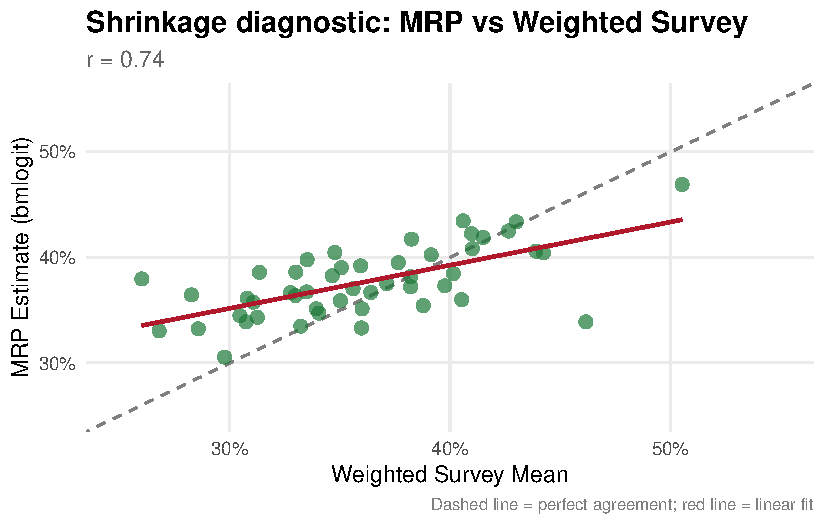
\includegraphics[keepaspectratio]{StateMRPpublicschools_files/figure-pdf/unnamed-chunk-9-1.pdf}}

\pandocbounded{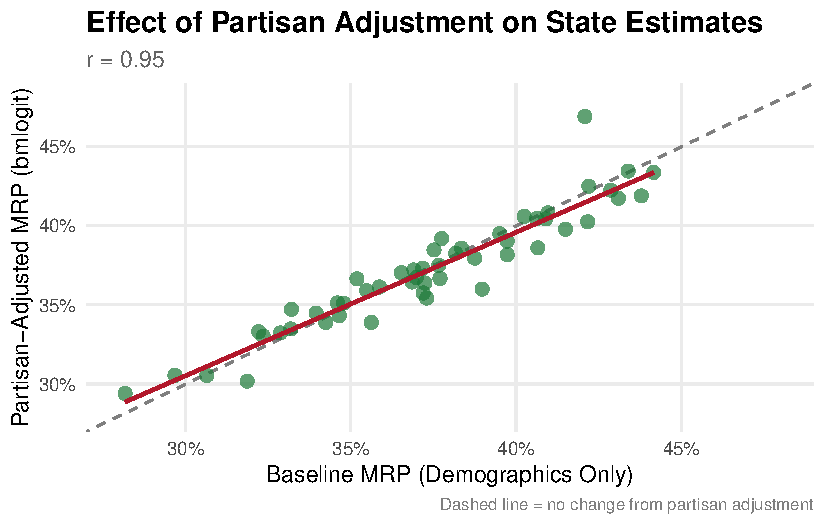
\includegraphics[keepaspectratio]{StateMRPpublicschools_files/figure-pdf/unnamed-chunk-9-2.pdf}}

Test for minorities about school integration.




\end{document}
